\chapter{Sobre \rc}

\section{Descripción del problema}
\label{problem_desc}

% Como nace el proyecto RecAbs ? Que necesitaba FuDePAN ?
El desarrollo de \rc{} surge como necesidad de \fude, la cuál es una organización no gubernamental sin fines de lucro que
realiza investigaciones en el campo de la bioinformática. Era menester de la fundación la implementación de una librería que facilitara la
solución a un gran número de proyectos bioinformáticos, los cuales usan a la recursión como mecanismo fundamental y poseen muchos factores
de implementación en común.

% Meta del proyecto
La meta de este proyecto es identificar una abstracción genérica con una estructura común a todas las soluciones recursivas a estos
problemas de interés y, al mismo tiempo, proveer una solución algorítmicamente eficiente para dichos proyectos. Esta abstracción abarca la
familia de problemas que cumplen las siguientes condiciones:
\begin{itemize}
    \item   la solución se adapte a un modelo recursivo. No obstante, se ajusta principalmente a aquellos problemas con definición
            inherentemente recursiva; y
            % Donde el árbol de recursión contenga sub-soluciones (nodos) cada vez más pequeños hasta llegar a un caso base (hojas).
            % Solucion recursiva natural
    \item   haya independencia de datos entre los nodos del árbol de recursión de la solución.
            % los nodos del árbol de recursión de la solución sean independientes.
\end{itemize}

Es importante aclarar que en \rc, la solución del problema a resolver debe adoptar la forma recursiva, donde el paso inductivo nos conduce a
problemas cada vez mas pequeños que necesariamente terminarán en, por lo menos, un caso base. También es significativo el segundo punto, el
cual expresa que sólo se pueden solucionar problemas con la recursividad mas simple, llegado a una hoja (caso base) se termina con esa rama
retornando un resultado sin poder volver atrás buscando diferentes caminos, como algoritmos backtracking, combinatorios, etc.

La librería permite lograr que usuarios sin altos conocimientos de programación solucionen problemas (en la mayoría de los casos
problemas temporalmente complejos en bioinformática) desconociendo sobre distribución entre servidor y clientes, administración de
clientes, balanceo de carga, manejo de resultados, y demás aspectos sobre computación distribuida.

% FuD-acoplando
Otra parte del problema fue la de acoplar \rc{} como una nueva capa del framework \fud. Esto es fundamental ya que la mayoría de los
problemas bioinformáticos requieren un nivel de procesamiento elevado, cómputos que en una sola computadora se hacen inmanejables. En la
sección \ref{sec:fud} se explican las partes básicas de este framework y más adelante hablaremos sobre los cambios de diseño que sufrió
para poder adaptar \rc.

\section{¿Qué es \rc?}

\rc{} es un nivel más en la pila de capas que conforma a \fud, como se explico anteriormente, este framework distribuye
automáticamente trabajo especificado en la tercer capa. \rc{} es una implementación genérica de la capa
\textit{aplicación} de \fud{} que abarca todas las soluciones recursivas a los problemas mencionados anteriormente en
\ref{problem_desc}. Con las restricciones previamente mencionadas \rc{} define una interfaz clara y sencilla para que un
usuario pueda implementar sus aplicación recursiva independizándose de todas aquellas tareas involucradas en computación
distribuida, como la división de trabajo, administración de clientes, recolección de resultados, balanceo de carga, etc.
Particularmente este proyecto hace hincapié en lograr un buen balanceo de carga en los nodos conectados.

\section{Funcionamiento de \rc}

% Arquitectura cliente-servidor
\rc{} tiene arquitectura \textbf{cliente-servidor}, por lo que tendremos dos aplicaciones: \textit{Cliente} y \textit{Servidor}.
Este modelo es una forma de computación distribuida en la que existe una relación \textit{Master-Worker}, ya que el servidor (master) está
encargado de llevar a cabo el progreso general del sistema y los clientes (workers) son los que procesan datos.

% 1 servidor, N clientes. Centralización y escalabilidad.
En un proyecto \rc{} debe haber solamente un servidor y $N$ clientes conectados al mismo. Esto permite, entre otras cosas, una
centralización del control de recursos e integridad de datos en el server y una excelente escalabilidad aumentando capacidad y número de
clientes.

% A continuación
Para entender la noción principal de cómo funciona una aplicación \rc{} se darán a continuación las partes fundamentales y la terminología
general del proyecto.

\subsection{Functor recursivo}
\label{functor}

% El functor recursivo
Es una abstracción de la \textit{función recursiva} de una aplicación concreta que se ejecutará sobre \rc. Describe un
estado particular así como también su comportamiento y responsabilidad. Esta información es específica de cada
aplicación, la cual es necesaria y suficiente para ser procesada por los clientes.

\subsection{Asistente del Servidor}
\label{server_helper}

% El asistente del Servidor
También es un concepto que el usuario deberá especificar a fines de informar a \rc{} detalles de como iniciar el
procesamiento y manipular mensajes. Las responsabilidades de este módulo son las siguientes:

\begin{itemize}
    \item   brindar el \textit{functor} inicial,
    \item   definir que hará con los resultados a medida que lleguen, y
    \item   definir el tratamiento de los mensajes intermedios (si es que los hubiera).
\end{itemize}
De estos requisitos, el primero es obligatorio y los dos restantes son opcionales en la medida de que la aplicación arroje resultados y
mensajes intermedios.

\subsection{Administrador de la Recursión}
\label{rmanager}
Este componente es el encargado de iniciar la ejecución total de cualquier proyecto que use la librería y depende del
\textit{middleware} de distribución concreto que se use, por ejemplo y en nuestro caso: \fud. Pero la tarea principal de
éste es la de accionar como un conmutador de paquetes, es el ``handler'' del lado servidor. Cada paquete que sale de un
cliente y, por lo tanto, llega a este \textit{manager} puede ser alguno de los siguientes tipos de paquete:

\begin{itemize}
    \item   un \textbf{resultado}, parcial y relativo a la unidad de trabajo que se procesó, el cuál es tratado de la
        manera que el usuario desee. Indica, en el cliente, que se ha llegado a una hoja en el árbol de recursión
        perteneciente al mismo.
    \item   un \textbf{mensaje intermedio} es cualquier dato transmitido de cliente a servidor sin llegar a una hoja o
        estado final en el árbol, y por lo tanto no es un resultado. También es enviado (en cliente) y tratado (en
        servidor) como el usuario disponga.
    \item   una \textbf{unidad de trabajo} a distribuir, la cuál será enviada a un cliente ocioso. Un \textit{trabajo}
        arribado es una partición del trabajo del cliente que lo envió.
\end{itemize}

\subsection{Asistente del Cliente}
\label{client_helper}

% El asistente del Cliente
\texttt{L4ClientApp} define la cantidad y/o tiempo en el que los clientes deben enviar los resultados y mensajes intermedios al server. El
desarrollador deberá o bien elegir una forma pre-establecida de envío o bien crear una propia. Si esta interfaz no es implementada, se
utiliza por default el envío de paquetes por tamaño fijo (actualmente establecida en 10 kilobytes).

\subsection{Procesador Recursivo}
\label{RProcessor}
Módulo que se encarga de llevar a cabo el procesamiento total de un functor en un nodo. Esto implica administrar la
reproducción de los functores hijos y su futura distribución o su ejecución local, permitir el envío de mensajes
y resultados al servidor, finalizar el proceso recolectando todos aquellos functores que se encuentren en caso base y
enviarlos al servidor. Es un componente de suma importancia ya que concentra gran parte de la lógica de \rc{} en lado
cliente.

\subsection{Política de Distribución}
\label{distribution_policy}

Es una interfaz que ofrece varios ``sabores'' de distribución ya implementados, así como la posibilidad de extender este conjunto de
políticas si el desarrollador quisiese. Cada política establece cuándo un cliente debe distribuir o cuándo debe parar y, en caso positivo,
cuánto debe distribuir. Cuando hablamos de \textit{distribuir}, hacemos referencia al envío de unidades de trabajo pendientes que los
clientes hacen con el fin de aprovechar la disponibilidad de clientes ociosos, y así poder lograr un buen \textit{balanceo de carga}.


\subsection{Dinámica de procesamiento}\label{dinamic_recabs}
A continuación se describe de una manera macroscópica las tres actividades más importante que realiza \rc{} a la
hora de resolver un problema concreto.

    \subsubsection{Inicio en Servidor}
        Interacción entre los componentes del servidor en el inicio del procesamiento. Aquí se muestra como el functor
        recursivo inicial es construido y enviado hacia algún cliente vía \fud{}.
       
        \begin{figure}[!ht]
            \begin{center}
                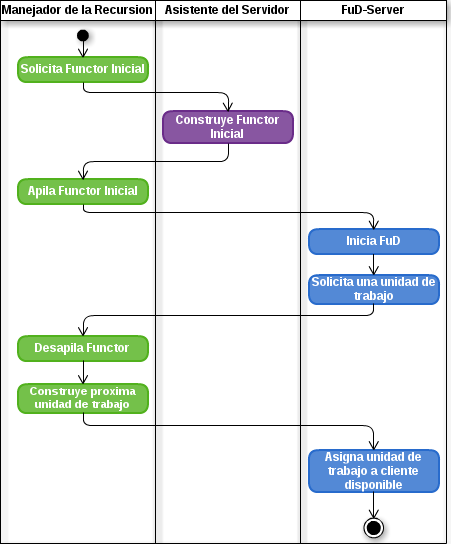
\includegraphics[scale=0.75]{images/ActivityRecAbs-1.png}
            \end{center}
            \caption{Diagrama de Actividades de inicio en servidor}
            \label{activity1}
        \end{figure}

    \subsubsection{Procesamiento en Cliente}
    En \ref{activity2} se ilustra mediante un diagrama de actividad el hilo de ejecución de un functor que llega a un
    cliente hasta su realización total, teniendo en cuenta también los casos en los que el cliente desee enviar
    resultados o mensajes en medio del proceso.

        \begin{figure}[!ht]
            \begin{center}

            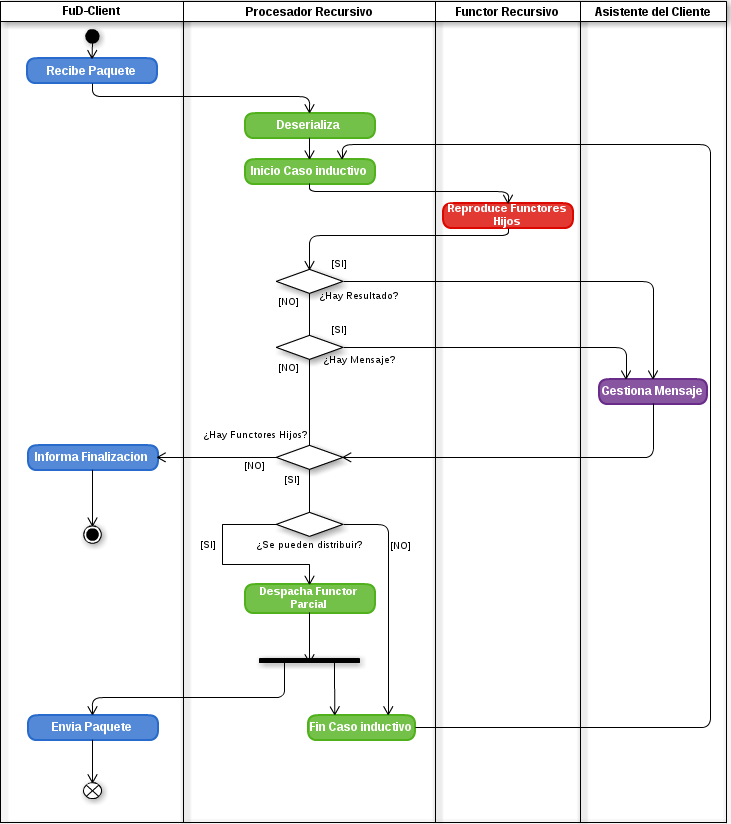
\includegraphics[scale=0.55]{images/ActivityRecAbs-2.png}
            \end{center}
            \caption{Diagrama de Actividades del procesamiento en Cliente}
            \label{activity2}
        \end{figure}


     \subsubsection{Recepción mensajes}
        Cada vez que \fud{} reciba un paquete, \rc{} analizará su tipo y tratará según corresponda. En caso de que
        lo arribado sea un mensaje o un resultado es el asistente quién se hará cargo, pero en cambio si lo que llega
        es otro functor recursivo resuelto parcialmente se apilará nuevamente para una futura distribución. 

            \begin{figure}[!ht]
                \begin{center}
                    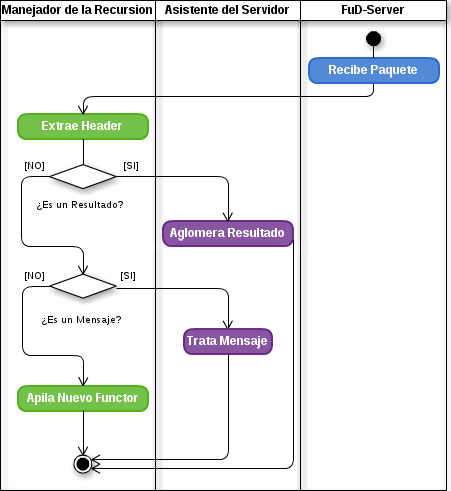
\includegraphics[scale=0.8]{images/ActivityRecAbs-3.png}
                    \end{center}
                    \caption{Diagrama de Actividades de recepción de mensajes}
                \label{activity3}
            \end{figure}

    \subsection{Aplicación}
        Para unificar todos los conceptos anteriores, la aplicación concreta deberá, en lado servidor, instanciar un
        Manejador de Recursión concreto, arrancarlo y luego informar los resultados. Por su parte, en el lado cliente,
        se deberá construir un procesador de recursión concreto e iniciarlo. Para mas detalles de como implementar y
        montar una aplicación concreta sobre \rc{} véase el capítulo \ref{chap:dummy_application}.


\section{Dependencias Externas}

Además de las bibliotecas STL (Standard Template Library) de cpp, recabs depende de otras bibliotecas, que se enuncian a continuación.

\subsection{MiLi}
\label{mili}

MiLi es una colección de pequeñas bibliotecas C++, compuesta únicamente por \textit{headers}. Sin necesidad de instalación, sin un
\textit{makefile}, sin complicaciones. Soluciones simples para problemas sencillos.

Esta biblioteca provee varias funcionalidades pequeñas en archivos cabecera (más conocidos como \textit{header files} en el ámbito de C/C++,
extensión ``.h'' o ``.hpp''), y puede ser descargada junto con su documentación en:
\begin{center}
    \texttt{http://mili.googlecode.com/}
\end{center}

MiLi ha sido utilizada extensamente a lo largo del desarrollo de  donde particularmente se destacan las funcionalidades provistas por
\textit{binary-streams} y \textit{container-utils}.

\begin{itemize}
    \item   \textbf{binary-streams:} esta biblioteca provee soporte a streams manejando información de cualquier tipo de objeto similar a
            como lo hace la biblioteca de entrada/salida estándar. En la Tabla \ref{bstreamuse} se muestra un ejemplo de su uso.
    \item   \textbf{container-utils:} esta biblioteca provee un conjunto de funciones, optimizadas para cada tipo de contenedor STL.
\end{itemize}

\begin{table}[!ht]
    \lstset{language=C++}
    \begin{lstlisting}[frame=single]
#include <iostream>
#include <string>
#include <vector>
#include "include/mili.h"

int main()
{
    std::vector<int> v(5,3); //all 3's
    v[1] = 1;
    v[4] = 7; //so it is [3,1,3,3,7]

    bostream bos;
    bos << 1 << 2 << 3 << std::string("Hello ") << v << 4 << std::string("World!");

    bistream bis(bos.str());

    int         nums[4];
    std::string str1;
    std::string str2;

    std::vector<int> v2;


    bis >> nums[0] >> nums[1] >> nums[2] >> str1 >> v2 >> nums[3] >> str2;

    for (int i=0; i < 4 ; ++i)
        std::cout << nums[i] << std::endl;

    std::cout << str1 << str2 << std::endl;

    std::cout << '[';
    for (size_t i=0; i < 5; ++i)
        std::cout<< v2[i] << ' ';
    std::cout << ']' << std::endl;
}
    \end{lstlisting}
    \centering \caption{C\'odigo extra\'ido de Mili::binary\_streams.}
    \label{bstreamuse}
\end{table}

\begin{table}[!htb]
    \lstset{language=C++}
    \begin{lstlisting}[frame=single]
#include <iostream>
#include <vector>
#include <string>
#include <queue>
#include "mili/mili.h"
using namespace std;

template <class T>
static void insert_elements(T& container);

int main()
{
    vector<int> v;
    v.push_back(1);
    map<string, string> m;
    m["hello"] = "good bye";
    m["Bonjour"] = "au revoir";
    m["hola"] = "adios";
    m["buenas"] = "adios";

    try
    {
        cout << contains(v, 2) << endl;         // will print 0 (false)
        cout << contains(m, "nothing") << endl; // will print 0

        cout << "map: " << endl;
        cout << remove_first_from(m, "au revoir") << endl; // will print 1
        cout << remove_all_from(m, "adios") << endl;       // will print 1

        cout << find(v, 1) << endl;         // will print 1 (true)
        cout << find(m, "hello") << endl;   // will print "good bye"
        cout << find(m, "world") << endl;   // will throw ElementNotFound
    }
    catch (ElementNotFound)
    {
        cerr << "Element not found!" << endl;
    }

    /* TEST - queue in container_utils::insert_into */
    queue<int> myqueue;
    insert_elements(myqueue);

    return 0;
}

template <class T>
static void insert_elements(T& container)
{
    insert_into(container, 100);
    insert_into(container, 100);
    insert_into(container, 100);
    insert_into(container, 200);
    insert_into(container, 300);
    insert_into(container, 400);
    insert_into(container, 400);
}
    \end{lstlisting}
    \centering \caption{C\'odigo extra\'ido de Mili::container\_utils.}
\end{table}
